\minitoc 

On s'intéresse dans ce chapitre et les suivants à la modélisation de l'éclairage sur une scène déjà modélisée numériquement. 
L'intérêt est de distribuer de façon réaliste une partie du spectre électromagnétique généré par une source de lumière sur les objets pour générer des images réalistes. 
On se base pour cela sur les propriétés physiques des matériaux représentés pour estimer numériquement leurs interactions avec la lumière. Théoriquement, on se basera sur des équations aux dérivées partielles décrivant ces interactions. Nous les résoudrons ensuite via des méthodes numériques, notament par des méthodes de Monte-Carlo. 

% ============================================================
% Grandeurs radiométriques fondamentales 

\section{Grandeurs radiométriques fondamentales}

Avant de parler d'équation du transfert radiatif, commençons par définir correctement les grandeurs physiques utilisées pour la description des interactions du spectre électromagnétique avec la matière. 

% ---------------------------------------------
\subsection{Principe du rendu}

On modélise ces interactions simplement par trois éléments : la source, la matière et le détecteur représentés en Figure~\ref{fig:chaine_rendu_principe}. 
Un signal $ \mathcal{E}$ est émis par une source lumineuse (soleil, ampoule) et est transporté sous la forme de rayonnements jusqu'aux objets de la scène. On définit alors un \emph{opérateur de transport} $ \mathcal{T}$ décrivant l'interaction de ce signal avec la matière (absorption, réflexion). Enfin un capteur (caméra, oeil) acquiert le signal reçu $ \mathcal{S} = \mathcal{T} \cdot \mathcal{E}$. En fonction de sa sensibilité à chaque longueur d'onde $ \mathcal{V}$, celui le capte différement, on obtient donc l'équation suivante : 
\begin{equation}
    \mathcal{R} = \int \mathcal{V}( \lambda) \cdot \mathcal{S}( \lambda) \mathrm{d} \lambda. 
\end{equation}

\begin{figure}[htbp]
    \centering
    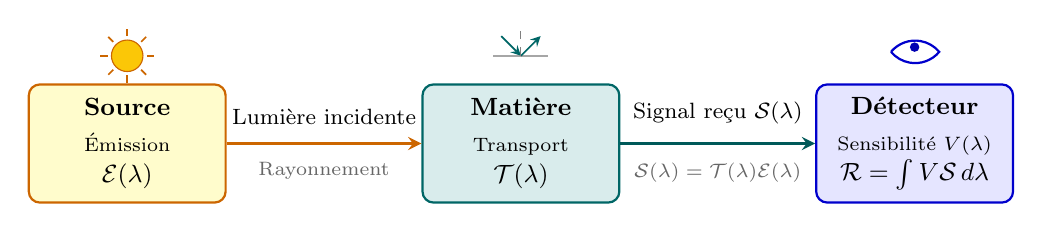
\begin{tikzpicture}[
        node distance=5cm,
        block/.style={
            draw, 
            rounded corners=4pt, 
            line width=0.8pt, 
            minimum width=2.5cm, 
            minimum height=1.5cm, 
            align=center, 
            font=\small
        },
        ray/.style={
            ->, 
            >=stealth, 
            very thick, 
            line width=1.1pt
        }
    ]
        % --- 1. Source de lumière ---
        \node[block, fill=yellow!20, draw=orange!80!black] (source) {
            \textbf{Source}\\[2pt]
            \scriptsize Émission\\
            $\mathcal{E}(\lambda)$
        };

        % --- 2. Objet / Interaction avec la matière ---
        \node[block, fill=teal!15, draw=teal!80!black, right of=source] (object) {
            \textbf{Matière}\\[2pt]
            \scriptsize Transport\\
            $\mathcal{T}(\lambda)$
        };

        % --- 3. Détecteur / Capteur (Œil / Caméra) ---
        \node[block, fill=blue!10, draw=blue!80!black, right of=object] (sensor) {
            \textbf{Détecteur}\\[2pt]
            \scriptsize Sensibilité $V(\lambda)$\\
            $\mathcal{R} = \int V\mathcal{S}\,d\lambda$
        };

        % --- Rayons lumineux et annotations aérées ---
        % Rayon incident
        \draw[ray, orange!80!black] (source) -- (object) 
            node[midway, above=3pt, font=\footnotesize, text=black] {Lumière incidente}
            node[midway, below=3pt, font=\scriptsize, text=gray!80!black] {Rayonnement};

        % Rayon réfléchi / transporté
        \draw[ray, teal!70!black] (object) -- (sensor) 
            node[midway, above=3pt, font=\footnotesize, text=black] {Signal reçu $\mathcal{S}(\lambda)$}
            node[midway, below=3pt, font=\scriptsize, text=gray!80!black] {$\mathcal{S}(\lambda) = \mathcal{T}(\lambda)\mathcal{E}(\lambda)$};

        % --- Icônes minimalistes géométriques ---
        % Soleil schématisé
        \begin{scope}[shift={(source.north)}, yshift=0.35cm]
            \draw[fill=yellow!60!orange, draw=orange!80!black] (0,0) circle (0.2cm);
            \foreach \a in {0, 45, 90, 135, 180, 225, 270, 315} {
                \draw[orange!80!black, semithick] (\a:0.25cm) -- (\a:0.34cm);
            }
        \end{scope}

        % Symbole de réflexion surfacique
        \begin{scope}[shift={(object.north)}, yshift=0.35cm]
            \draw[thick, gray!70] (-0.35, 0) -- (0.35, 0);
            \draw[->, >=stealth, semithick, teal!80!black] (-0.25, 0.25) -- (0, 0);
            \draw[->, >=stealth, semithick, teal!80!black] (0, 0) -- (0.25, 0.25);
            \draw[thin, dashed, gray] (0, 0) -- (0, 0.35);
        \end{scope}

        % Symbole de capteur / œil
        \begin{scope}[shift={(sensor.north)}, yshift=0.4cm]
            \draw[thick, blue!80!black] (-0.3, 0) arc (140:40:0.4) arc (-40:-140:0.4);
            \fill[blue!70!black] (0, 0.06) circle (0.06);
        \end{scope}
    \end{tikzpicture}
    \caption{Chaîne fondamentale de formation de l'image en synthèse d'images : de l'émission à la réponse du capteur.}
    \label{fig:chaine_rendu_principe}
\end{figure}

L'objectif du rendu est de modéliser l'ensemble de ces notions physiques. La principale difficulté est dans l'estimation du transport $ \mathcal{T}$. On considèrera pour cela les interactions \emph{microscopiques} (entre les photons et la structure atomique du matériaux) et les interactions \emph{macroscopiques}. 

Pour cela, on développera des modèles statistiques macroscopiques basés sur les propriétés microscopiques des matériaux : on parlera de \emph{modèles hybrides}. 

% ---------------------------------------------
\subsection{De l'angle 2D à l'angle solide}

Nous posons ici les définitions fondamentales de la radiométrie. Intuitivement, on part de la puissance d'un rayonnement émis et on essaye de décrire ses interactions avec la matière en fonction de son angle incident ainsi que la quantité de surface (aire) interceptée. 

\begin{definition}[Angle solide]
    Pour quantifier la partition de l'espace visuel sous-tendue par un objet vu depuis un point quelconque, on défini la notion \emph{d'angle solide}. 
    Pour cela, on projette l'objet sur une sphère de rayon $r$ centrée sur le point de vue, on obtient alors l'expression de la surface de la sphère interceptée à partir de l'aire couverte par le rayonnement et son rayon : 
    \begin{equation}
        \dd \omega = \frac{ \dd A_{\text{sphère}}}{r^2}
    \end{equation}
    exprimé en stéradians ($ \mathrm{sr}$). En utilisant les coordonnées sphériques, pour une petite variation $\dd \theta$ de la colatitude $ \theta$ et une variation $ \dd \varphi$ de la longitude $ \varphi$, on a la formule suivante : 
    \begin{equation}
        \dd \omega = \sin \theta \dd \theta \dd \varphi. 
    \end{equation} 
    Dans le cas d'une surface dont la normale fait un angle $ \theta$ avec la direction d'observation, alors l'aire induite n'est que de $ \dd A \cos \theta$, on peut alors approximer l'angle solide par : 
    \begin{equation}
        \dd \omega \simeq \frac{\dd A \cos \theta}{r^2}. 
    \end{equation}
\end{definition}

\begin{proposition}
    % TODO : Décrire les calculs pour les angles solides
\end{proposition}

% ---------------------------------------------
\subsection{Grandeurs physiques}

Les angles solides permettent ensuite de définir de nouvelles notions et grandeurs physiques permettant de décrire le comportement du spectre électromagnétique. Ici, on commence donc par proposer quelques métriques permettant de quantifier l'énergie émise par une source (flux et intensité rayonnante) puis on présente des métriques quantifiant le rayonnement reçu ou réfléchit par des surfaces. 

\begin{definition}[Puissance Rayonnante - Flux]
    On appelle \emph{puissance rayonnante} ou \emph{flux} $P$ (ou $ \Phi$) l'énergie totale émise, transportée ou reçue par unité de temps. Elle s'exprime en Joules par secondes dont l'unité internationnale est le Watts. 
\end{definition}

\begin{definition}[Intensité rayonnante]
    On considère une source ponctuelle émettant de l'énergie par rayonnement d'une puissance $P$. On s'intéresse à la quantité d'énergie qu'elle distribue dans la direction $ \dd \omega$ d'un angle solide. Cette dernière est appelée \emph{intensité rayonnante} et est définie par : 
    \begin{equation}
        I = \frac{\dd P}{\dd \omega} \quad [\mathrm{W} \cdot \mathrm{sr}^{-1}]
    \end{equation}
    Elle s'exprime en Watts par stéradians. Si la source émet la même quantité d'énergie dans toutes les directions, on dit qu'elle est \emph{isotrope} et on a $I = \frac{P}{4 \pi}\; \mathrm{W} \cdot \mathrm{sr}^{-1}$. 
\end{definition}

On peut maintenant s'intéresser à la quantité d'énergie acquise ou émise par une surface quelconque. On défini pour cela l'exitance et l'irradiance. 

\begin{definition}[Exitance -- Irradiance]
    Soit une surface $ \dd A$ émettant du rayonnement de flux $ P_{\text{émis}}$ et recevant un rayonnement de flux $ P_{\text{reçu}}$. On peut alors définir la densité surfacique de rayonnement qui quitte la surface, appelée \emph{exitance} : 
    \begin{equation}
        M = \frac{P_{\text{émis}}}{\dd A} \quad [\mathrm{W} \cdot \mathrm{m}^{-2}]. 
    \end{equation}
    De même, on définit la densité surfacique de rayonnement qui arrive sur la surface par \emph{l'irradiance} : 
    \begin{equation}
        E = \frac{P_{\text{reçu}}}{\dd A} \quad [\mathrm{W} \cdot \mathrm{m}^{-2}]. 
    \end{equation}
\end{definition}

Ces trois dernières grandeurs nous permettent de quantifier une quantité de rayonnement par rapport à une surface précise (exitance/irradiance) ou une direction donnée (intensité rayonnante). On souhaiterait maintenant combiner les deux : quantifier la puissance émise/reçu par une surface donnée dans une direction donnée, c'est la \emph{radiance}. 

\begin{definition}[Radiance/Luminance]
    Soit un objet de surface $ \dd A$, une direction donnée par l'angle solide $ \dd \omega$ et une intensité $I$. On défini la \emph{radiance} (ou luminance) de cette surface dans la direction $\dd \omega$ par : 
    \begin{equation}
        L = \frac{\dd[2]{P}}{\dd A \cos \theta \dd \omega} \quad [\mathrm{W} \cdot \mathrm{m}^{-2} \cdot \mathrm{sr}^{-1}]
    \end{equation}
\end{definition}

\begin{remark}
    La radiance est invariante dans le vide en position. En effet pour un observateur d'une surface $ \dd A$, la quantité de rayonnement (intensité) qui part dans sa direction $ \dd \omega$ depuis la surface est égale à celle qu'il reçoit. 
    D'autre part, la réponse du capteur est proportionnelle à la radiance du corps qu'il observe. 
\end{remark}

\begin{proposition}[Transfert radiatif]
    Soient deux éléments de surfaces dont une source $ \dd A_1$ et un récepteur $ \dd A_2$ séparés par une distance $r$ représentés dans la Figure~\ref{fig:transfert_radiatif_surfaces}. On suppose que la source émet de la radiance $L$ sous un angle $ \theta_1$ par rapport à la direction (en bleu). Le récepteur $ \dd A_2$ sous-tend depuis $ \dd A_1$ un angle solide $\dd \omega_1$ tel que : 
    \begin{equation}
        \dd \omega_1 = \frac{\dd A_2 \cos \theta_2}{r^2}. 
    \end{equation}
    En réinjectant $ \dd \omega_1$ dans la formule de la radiance $ \dd[2]{P} = L \cdot \dd A_1 \cdot \cos \theta_1 \dd \omega_1$, on obtient l'expression du transfert élémentaire d'énergie entre les deux surfaces : 
    \begin{equation}
        \dd[2]{P} = L \frac{\cos \theta_1 \cos \theta_2}{r^2} \dd A_1 \dd A_2
        = L \cdot G(x_1, x2) \cdot \dd A_1 \dd A_2. 
    \end{equation}
    Où l'on note $G(x_1, x_2) = \frac{ \cos \theta_1 \cos \theta2}{\|x_1 - x_2 \|^2}$ le \emph{terme géométrique}. 
\end{proposition}

\begin{figure}[htbp]
    \centering
    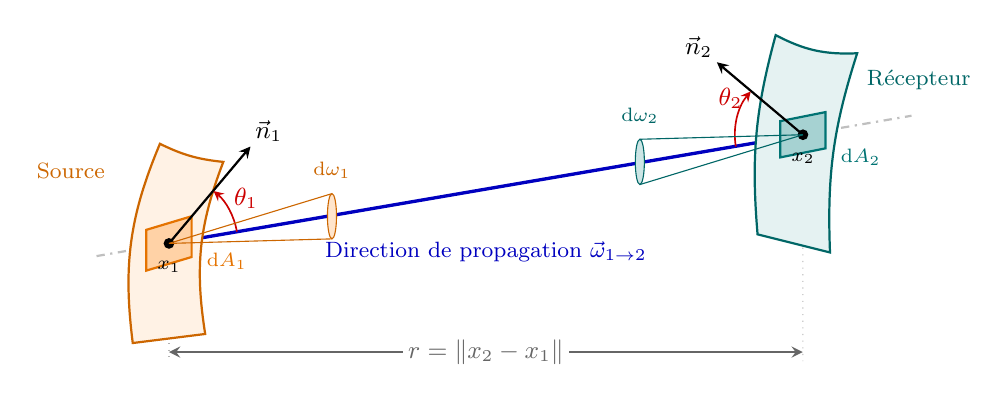
\begin{tikzpicture}[scale=1.15, >=stealth]
        % --- Définition des coordonnées centrales des facettes ---
        \coordinate (x1) at (0, 0);       % Centre de dA1 (Source)
        \coordinate (x2) at (7, 1.2);     % Centre de dA2 (Récepteur)

        % --- Axe optique direct (direction de propagation) ---
        % Angle de la ligne de visée x1 -> x2 : ~ 9.73°
        \draw[thick, dashdotted, gray!50] (-0.8, -0.14) -- (8.2, 1.41);
        \draw[very thick, ->, blue!75!black] (x1) -- (x2) 
            node[midway, below=15pt, font=\footnotesize] {Direction de propagation $\vec{\omega}_{1\to 2}$};

        % Cotation de la distance r
        \draw[<->, thick, gray!80!black] (0, -1.2) -- (7, -1.2)
            node[midway, fill=white, inner sep=2pt, font=\small] {$r = \|x_2 - x_1\|$};
        \draw[dotted, gray!60] (x1) -- (0, -1.3);
        \draw[dotted, gray!60] (x2) -- (7, -1.3);

        % ==============================================================
        % SURFACE 1 : Émetteur (Source dA1)
        % ==============================================================
        % Patch courbé source (centré en x1 = (0,0))
        \draw[thick, fill=orange!10, draw=orange!80!black] 
            (-0.4, -1.1) to[bend left=15] (-0.1, 1.1) 
                         to[bend right=10] (0.6, 0.9) 
                         to[bend right=15] (0.4, -1.0) -- cycle;
        \node[font=\footnotesize, orange!80!black, left] at (-0.6, 0.8) {Source};

        % Facette différentielle dA1 parfaitement centrée sur x1
        \draw[thick, fill=orange!35, draw=orange!90!black] 
            (-0.25, -0.3) -- (0.25, -0.15) -- (0.25, 0.3) -- (-0.25, 0.15) -- cycle;
        \filldraw[black] (x1) circle (1.5pt) node[below=3pt, font=\scriptsize] {$x_1$};
        \node[font=\scriptsize, orange!90!black, right=2pt] at (0.25, -0.2) {$\mathrm{d}A_1$};

        % Normale n1 (inclinée vers la direction de x2, angle ~ 50°)
        \coordinate (n1_end) at (0.9, 1.07);
        \draw[thick, ->, black] (x1) -- (n1_end) node[above right=-2pt, font=\small] {$\vec{n}_1$};

        % Arc pour l'angle theta 1 (entre axe 9.7° et n1 50°)
        \draw[->, semithick, red!80!black] (0.75, 0.13) arc (9.7:50:0.75);
        \node[red!80!black, font=\small] at (0.85, 0.5) {$\theta_1$};

        % Cône d'angle solide d\omega_1
        \coordinate (c1_top) at (1.8, 0.55);
        \coordinate (c1_bot) at (1.8, 0.05);
        \draw[thin, orange!80!black] (x1) -- (c1_top);
        \draw[thin, orange!80!black] (x1) -- (c1_bot);
        \draw[thin, fill=orange!20, draw=orange!80!black] (1.8, 0.3) ellipse (0.05 and 0.25);
        \node[font=\scriptsize, orange!80!black, above=2pt] at (1.8, 0.55) {$\mathrm{d}\omega_1$};

        % ==============================================================
        % SURFACE 2 : Récepteur (dA2)
        % ==============================================================
        % Patch courbé récepteur (centré en x2 = (7, 1.2))
        \draw[thick, fill=teal!10, draw=teal!80!black] 
            (6.5, 0.1) to[bend left=10] (6.7, 2.3) 
                       to[bend right=15] (7.6, 2.1) 
                       to[bend right=10] (7.3, -0.1) -- cycle;
        \node[font=\footnotesize, teal!80!black, right] at (7.6, 1.8) {Récepteur};

        % Facette différentielle dA2 parfaitement centrée sur x2
        \draw[thick, fill=teal!35, draw=teal!90!black] 
            (6.75, 0.95) -- (7.25, 1.05) -- (7.25, 1.45) -- (6.75, 1.35) -- cycle;
        \filldraw[black] (x2) circle (1.5pt) node[below=3pt, font=\scriptsize] {$x_2$};
        \node[font=\scriptsize, teal!90!black, right=2pt] at (7.25, 0.95) {$\mathrm{d}A_2$};

        % Normale n2 (inclinée vers x1, angle ~ 140°)
        \coordinate (n2_end) at (6.05, 2.0);
        \draw[thick, ->, black] (x2) -- (n2_end) node[above left=-2pt, font=\small] {$\vec{n}_2$};

        % Arc pour l'angle theta 2 (entre axe retour 189.7° et n2 140°)
        \draw[->, semithick, red!80!black] (6.26, 1.07) arc (189.7:140:0.75);
        \node[red!80!black, font=\small] at (6.2, 1.6) {$\theta_2$};

        % Cône d'angle solide d\omega_2
        \coordinate (c2_top) at (5.2, 1.15);
        \coordinate (c2_bot) at (5.2, 0.65);
        \draw[thin, teal!80!black] (x2) -- (c2_top);
        \draw[thin, teal!80!black] (x2) -- (c2_bot);
        \draw[thin, fill=teal!20, draw=teal!80!black] (5.2, 0.9) ellipse (0.05 and 0.25);
        \node[font=\scriptsize, teal!80!black, above=2pt] at (5.2, 1.15) {$\mathrm{d}\omega_2$};

    \end{tikzpicture}
    \caption{Transport radiatif différentiel entre deux éléments de surface orientés $\mathrm{d}A_1$ et $\mathrm{d}A_2$ séparés par une distance $r$.}
    \label{fig:transfert_radiatif_surfaces}
\end{figure}

% ---------------------------------------------
\subsection{Distribution spectrale et émission thermique : le corps noir}

Les grandeurs précédement définies ne tenaient pas compte de la longueur d'onde d'émission/réception des objets ni de leur température. Or l'énergie transportée par un rayonnement en dépend fortement. L'introduction du principe du \emph{corps noir} permet justement de formaliser cette différence. 

En physique, un corps noir est un objet idéal qui absorbe tout le rayonnement reçu. Pour rester en équilibre thermodynnamique à une température $T$, il réémet cet excès d'énergie sous la forme de rayonnement spectral isotrope. 

\begin{definition}[Exitance du corps noir]
    La loi de Planck donne l'exitance monochromatique $M_\lambda^0$ (pour une longueur d'onde donnée) du corps noir : 
    \begin{equation}
        M_\lambda^0 = \frac{2 \pi h c^2}{ \lambda^5 \left( \exp \left( \frac{hc}{k \lambda T}\right) -1\right)} \quad [\mathrm{W} \cdot \mathrm{m}^{-2} \cdot \mathrm{nm}^{-1}]. 
    \end{equation}
    Où $h$ est la constante de Planck, $c$ la célérité de la lumière dans le vide, $k$ la constante de Boltzman et $T$ la température du corps en kelvin. 
\end{definition}

Cette équation défini la quantité de rayonnement émise par un corps noir à température constante pour une longueur d'onde donnée par unité de surface. 

\begin{proposition}[Radiance Spectrique]
    Comme le corps noir diffuse son surplus d'énergie de manière isotrope, on peut calculer sa radiance spectrique (radiance pour une longueur d'onde donnée) à l'aide de la relation $ M_\lambda^0 = \pi L_{\lambda, b}$. On a donc : 
    \begin{equation}
        L_{\lambda, b} = \frac{2 h c^2}{ \lambda^5 \left( \exp \left( \frac{hc}{k \lambda T}\right) -1\right)} \quad [\mathrm{W} \cdot \mathrm{m}^{-2} \cdot \mathrm{sr}^{-1} \cdot \mathrm{nm}^{-1}]. 
    \end{equation}
\end{proposition}

Dans une scène réelle, les matériaux ne se comportent pas comme des corps noirs parfaits : ils n'absorbent qu'une fraction du rayonnement incident et n'émettent qu'une partie du flux théorique prédit par la loi de Planck. On introduit alors des coefficients spectraux adimensionnels compris dans $[0, 1]$ pour caractériser leur comportement radiatif.

\begin{definition}[Émissivité, absorptivité et albédo]
    Pour un matériau donné à la température $T$ et pour une longueur d'onde $\lambda$ :
    \begin{itemize}
        \item L'\emph{émissivité} $\epsilon_\lambda \in [0, 1]$ est le rapport entre l'exitance réelle du matériau $M_\lambda$ et celle du corps noir équivalent $M_\lambda^0$ à la même température :
        \begin{equation}
            \epsilon_\lambda = \frac{M_\lambda}{M_\lambda^0} \in [0, 1].
        \end{equation}
        \item L'\emph{absorptivité} $\alpha_\lambda \in [0, 1]$ correspond à la fraction du flux énergétique incident absorbée par le matériau à la longueur d'onde $\lambda$.
        \item L'\emph{albédo} spectral (ou réflectance hémisphérique) $\rho_\lambda \in [0, 1]$ est la proportion du flux incident réfléchie par la surface.
    \end{itemize}
\end{definition}

\begin{proposition}[Loi de Kirchhoff et conservation de l'énergie]
    À l'équilibre thermodynamique local, la \emph{loi du rayonnement de Kirchhoff} établit que l'émissivité d'un corps est égale à son absorptivité pour chaque longueur d'onde :
    \begin{equation}
        \epsilon_\lambda = \alpha_\lambda.
    \end{equation}
    Dès lors, pour un matériau opaque (pour lequel aucune transmission interne n'a lieu, i.e. transmittance nulle), le principe fondamental de conservation de l'énergie impose $\rho_\lambda + \alpha_\lambda = 1$. On en déduit la relation liant la réflectance à l'émissivité :
    \begin{equation}
        \rho_\lambda = 1 - \alpha_\lambda = 1 - \epsilon_\lambda.
    \end{equation}
\end{proposition}

Cette formulation permet de paramétrer directement les termes sources et les propriétés de surface : un corps noir correspond au cas limite $\epsilon_\lambda = \alpha_\lambda = 1$ et $\rho_\lambda = 0$, tandis qu'un réflecteur idéal satisfait $\rho_\lambda = 1$ et $\epsilon_\lambda = 0$.

% ============================================================
% Équation des transferts radiatif & Équation du rendu

\section{Équation des transferts radiatif \& Équation du rendu}

Maintenant que nous avons posé le contexte de la modélisation de l'éclairage ainsi que les métriques nécessaires à sa description, nous pouvons nous intéresser à sa modélisation mathématique. 

% ---------------------------------------------
\subsection{Modélisation du capteur et de la caméra}

Au début de ce chapitre, nous avons fait l'hypothèse que le signal reçu par un capteur est de la forme : 
\begin{equation}
    \mathcal{R} = \int \mathcal{V}( \lambda) \cdot \mathcal{T}( \lambda) \cdot \mathcal{E}( \lambda)\mathrm{d} \lambda
\end{equation}
où $ \mathcal{T}$ est l'opérateur de transport du rayonnement, $ \mathcal{E}$ représente l'émission, $ \mathcal{V}$ la sensibilité du capteur et $ \mathcal{R}$ le signal reçu par ce dernier. 

\begin{proposition}
    Soit $S(x,y)$ le signal reçu par un pixel $(x,y)$ du capteur de la caméra. Pour que celui-ci reçoit de la lumière de la scène 3d, le signal doit traverser la lentille du capteur de surface $\mathcal{L}$ paramétrée par $(u,v)$ (ex: focale, largeur, etc...). Ainsi la quantité de lumière perçue par le capteur est le cumul de tous les rayons collectés sur l'étendue de la lentille $ \dd A(u,v)$ dans toutes les directions incidentes possibles $ \dd \omega_l$ pendant toute la durée de l'exposition $ \dd t$. 
    On peut donc modéliser ces notions par des applications : 
    \begin{itemize}
        \item $W(x, y, x_l, \omega_l, t)$ la fonction représentant le transfert optique de la lentille, 
        \item $L_i(x, y, \omega_l, t)$ est la radiance arrivant sur la lentille au point $x_l$, depuis la direction $\omega_l$, à l'instant $t$. 
    \end{itemize}
    On peut alors exprimer le signal reçu par le pixel $(x,y)$ du capteur :
    \begin{equation}
        S(x,y) = \int_T \int_\mathcal{L} \int_\Omega W(x, y, x_l, \omega_l, t) L_i(x, y, \omega_l, t) \dd \omega_l \dd A(u,v) \dd t. 
    \end{equation}
\end{proposition}

Or un pixel $P$ sur un écran n'est pas un point mathématique sans dimension : il correspond à une petite zone bidimensionnelle centrée en $(x_P, y_P)$. En réalité, le capteur physique intègre toute la lumière qui tombe sur sa zone sensible. De plus, en traitement du signal graphique, on applique un filtre de reconstruction noté $h_P$. L'intégrale du pixel s'écrit donc :
\begin{equation}
    I_p = \int_{s(h_P)} h_P(\Delta x, \Delta y) \, S(x_P + \Delta x, \, y_P + \Delta y) \, \mathrm{d}\mathcal{A}(\Delta x, \Delta y)
\end{equation}
où : 
\begin{itemize}
    \item $(\Delta x, \Delta y)$ est le décalage local par rapport au centre du pixel $(x_P, y_P)$.
    \item $s(h_P)$ : le support spatial du filtre (par exemple, un carré de $1 \times 1$ pixel pour un filtre boîte élémentaire, ou une zone de $2 \times 2$ pixels pour une gaussienne ou un filtre de Mitchell-Netravali).
    \item $h_P(\Delta x, \Delta y)$ : la fonction de pondération (le noyau du filtre). Elle donne plus d'importance aux rayons qui frappent le centre du pixel qu'à ceux qui touchent la périphérie. Pour conserver l'énergie, on a toujours $\int h_P = 1$.
    \item $\mathrm{d}\mathcal{A}(\Delta x, \Delta y)$ : l'élément d'aire infinitésimal sur la surface du pixel ($\mathrm{d}x\,\mathrm{d}y$). 
\end{itemize}

On peut donc maintenant se demander comment exprimer la radiance arrivant sur la lentille au point $x_i$. Celle-ci dépend directement de la géométrie de la scène et des propriétés de son éclairage. 

% ---------------------------------------------
\subsection{Formulation de l'ETR}

La section précédente s'est concentrée sur la modélisation physique de la réception d'un rayon par un capteur. Ici, on s'intéresse aux interactions de ce rayon dans l'environnement de la scène (air, eau, poussière). On appellera cette équation \emph{l'équation du transfert radiatif}. 

\begin{figure}[htbp]
    \centering
    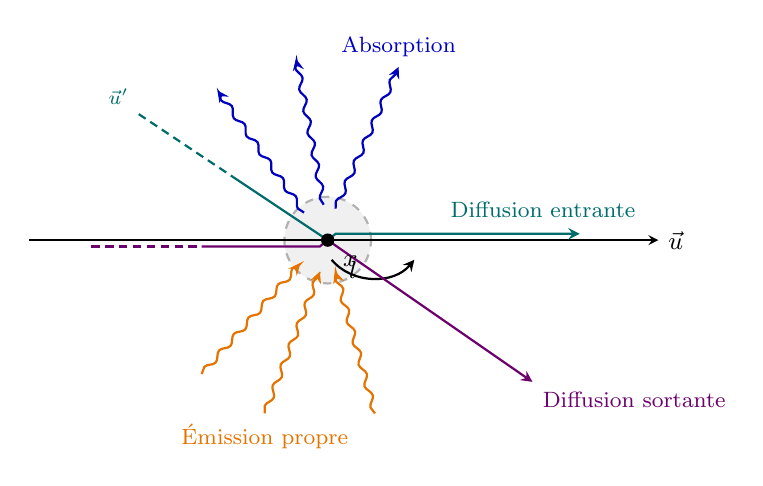
\begin{tikzpicture}[scale=1.0, >=stealth]
        % --- Définition du point central ---
        \coordinate (x) at (0, 0);

        % Cercle de contrôle : remplissage gris léger et contour en pointillés grisés
        \filldraw[fill=gray!12, draw=gray!60, dashed, thick] (x) circle (0.55);

        % --- Axe principal noir u (trait semithick) ---
        \draw[semithick] (-3.8, 0) -- (x);
        \draw[semithick, ->] (x) -- (4.2, 0) node[right, font=\small] {$\vec{u}$};

        % --- Arc de flèche représentant l'avancement dl le long de u ---
        \draw[thick, ->, black] (0.05, -0.25) to[bend right=50] (1.1, -0.25)
            node[at end, below right=4pt, font=\small] {$\dd l$};

        % ==============================================================
        % 1. DIFFUSION ENTRANTE (Vert émeraude / Teal)
        % ==============================================================
        \draw[thick, densely dashed, teal!85!black] (-2.4, 1.6) -- (-1.2, 0.8);
        \draw[thick, teal!85!black] (-1.2, 0.8) -- (x);
        \draw[thick, ->, teal!85!black] (x) -- (0.1, 0.08) -- (3.2, 0.08)
            node[pos=0.85, above=2pt, font=\footnotesize] {Diffusion entrante};
        \node[teal!85!black, font=\scriptsize, above left] at (-2.4, 1.6) {$\vec{u}'$};

        % ==============================================================
        % 2. DIFFUSION SORTANTE (Violet)
        % ==============================================================
        \draw[thick, densely dashed, violet!85!black] (-3.0, -0.08) -- (-1.6, -0.08);
        \draw[thick, violet!85!black] (-1.6, -0.08) -- (-0.1, -0.08) -- (x);
        \draw[thick, ->, violet!85!black] (x) -- (2.6, -1.8)
            node[below right, font=\footnotesize] {Diffusion sortante};

        % ==============================================================
        % 3. ABSORPTION (Bleu cobalt : flèches ondulées quittant x)
        % ==============================================================
        \draw[thick, ->, blue!75!black, decorate, decoration={snake, amplitude=1pt, segment length=8pt}] 
            (0.1, 0.4) -- (0.9, 2.2)
            node[above, font=\footnotesize] {Absorption};
        \draw[thick, ->, blue!75!black, decorate, decoration={snake, amplitude=1pt, segment length=8pt}] 
            (-0.3, 0.35) -- (-1.4, 1.9);
        \draw[thick, ->, blue!75!black, decorate, decoration={snake, amplitude=1pt, segment length=8pt}] 
            (-0.05, 0.45) -- (-0.4, 2.3);

        % ==============================================================
        % 4. ÉMISSION PROPRE (Orange cuivré : flèches ondulées convergeant vers x)
        % ==============================================================
        \draw[thick, ->, orange!90!black, decorate, decoration={snake, amplitude=1pt, segment length=8pt}] 
            (-0.8, -2.2) -- (-0.1, -0.4)
            node[below, at start, font=\footnotesize] {Émission propre};
        \draw[thick, ->, orange!90!black, decorate, decoration={snake, amplitude=1pt, segment length=8pt}] 
            (0.6, -2.2) -- (0.1, -0.4);
        \draw[thick, ->, orange!90!black, decorate, decoration={snake, amplitude=1pt, segment length=8pt}] 
            (-1.6, -1.7) -- (-0.35, -0.3);

        % Point central rempli de noir plein par-dessus les tracés
        \filldraw[fill=black, draw=black] (x) circle (2.2pt) 
            node[below right=2pt, font=\small] {$x$};
    \end{tikzpicture}
    \caption{Bilan des interactions locales de l'ETR en un point matériel $x$ sur l'élément de longueur $\dd l$ le long de la direction $\vec{u}$.}
    \label{fig:etr_bilan_interactions_simple}
\end{figure}

Soit un rayon lumineux $ \vec{u} $ traversant un milieu (voir Figure~\ref{fig:etr_bilan_interactions_simple}), on note $x$ un point de ce rayon et on s'intéresse à la variation de luminance de ce rayon pour une petite variation d'abscisse $ \dd l$ de $x$. On peut alors observer différentes interactions avec l'environnement :
\begin{itemize}
    \item \textbf{Absorption} : Une partie des photons composant le rayon sont absorbés par le milieu, notament lors de percussions avec des atomes, qui augmente le niveau d'énergie. C'est de l'énergie perdu pour le rayon $ \vec{u} $, elle s'exprime de la façon suivante : 
    \begin{equation}
        \left( \frac{\partial L_\lambda}{ \partial l}\right)_{\text{abs}} = - \kappa_\lambda L_\lambda(x \to \vec{u} ). 
    \end{equation}
    où $ \kappa_\lambda$ est le coefficient d'absorption du milieu en $ m^{-1}$. 
    \item \textbf{Diffusion sortante} : Des photons peuvent se propager dans le milieu dû à l'énergie environnante. Lorsqu'ils entrent en collision avec le rayon, certains photons de ce dernier peuvent être déviés et perdus dans le milieu. On exprime cette perte par : 
    \begin{equation}
        \left( \frac{ \partial L_\lambda}{ \partial l}\right)_{\text{diff, out}} = - \sigma_\lambda L_\lambda(x \to \vec{u})
    \end{equation}
    avec $ \sigma_\lambda$ le coefficient de diffusion du milieu en $m^{-1}$. 
    \item \textbf{Émission propre} : Le milieu n'étant pas vide et à une certaine température, ce surplus d'énergie est transféré sous la forme de rayonnement dont une partie est transmise au rayon $ \vec{u}$ :
    \begin{equation}
         \left( \frac{ \partial L_\lambda}{ \partial l}\right)_{\text{emis}} = \kappa_\lambda L_{\lambda, b}(x)
    \end{equation}
    avec $ L_{\lambda, b}(x)$ l'émission du corps noir. 
    \item \textbf{Diffusion entrante} :  À l'inverse, des photons du milieu percutant le rayon $ \vec{u} $ peuvent être déviés dans le direction de ce rayon, c'est donc de l'énergie gagnée. On a : 
    \begin{equation}
        \left( \frac{ \partial L_\lambda}{ \partial l}\right)_{\text{diff, in}} = \frac{ \sigma_\lambda}{4 \pi} \int_{4 \pi} L_\lambda (x \leftarrow \vec{u'} ) \Phi ( \lambda, \vec{u} , \vec{u'} ) \dd \omega( \vec{u'} )
    \end{equation}
    où $ \Phi ( \lambda, \vec{u} , \vec{u'} )$ est la fonction de phase (BRDF volumique) : elle normalise la probabilité qu'un photon venant d'un autre rayon $ \vec{u'} $ soit dévié par $ \vec{u} $. On intègre cette probabilité sur toute la sphère autour de $x$ pour prendre en compte tous les rayons possibles $ \vec{u'} $ du milieu. 
\end{itemize}

L'équation du transfert radiatif s'écrit alors simplement comme la somme de toutes ces variations. 

\begin{theorem}[ETR -- Chandrasekhar, 1960]
    L'équation du transfert radiatif dans le contexte posé précédement fut proposée par Chandrasekhar en 1960. Elle s'exprime sous la forme : 
    \begin{align}
        \frac{ \partial}{ \partial l} L_\lambda(x \to \vec{u} ) &= - ( \kappa_\lambda + \sigma_\lambda) L_\lambda(x \to \vec{u} ) + \kappa_\lambda L_{\lambda, b}(x) \\
        &+ \frac{ \sigma_\lambda}{4 \pi} \int_{4 \pi} L_\lambda (x \to \vec{u'} ) \Phi ( \lambda, \vec{u} , \vec{u'} ) \dd \omega( \vec{u'} ). 
    \end{align}
    On peut poser $k(s) = \kappa(s) + \sigma(s)$ représentant la perte par unité de longueur $ \dd l$. 
\end{theorem}

On peut en proposer une version plus condensé pour obtenir sa formulation canonique. 

\begin{definition}[Coefficient d'extinction et terme source volumique]
    Afin de condenser l'écriture différentielle, on regroupe les mécanismes selon leur nature (pertes proportionnelles au flux incident vs gains locaux) :
    \begin{itemize}
        \item Le \emph{coefficient d'extinction} $k_\lambda(x)$ quantifie l'atténuation totale subie par le faisceau par unité de longueur :
        \begin{equation}
            k_\lambda(x) = \kappa_\lambda(x) + \sigma_\lambda(x) \quad [\mathrm{m}^{-1}].
        \end{equation}
        \item Le \emph{terme source volumique} $L_{i, \lambda}(x \to \vec{u})$ regroupe l'ensemble de l'énergie thermique créée et de l'énergie ambiante rabattue vers la direction $\vec{u}$ par le milieu :
        \begin{equation}
            L_{i, \lambda}(x \to \vec{u}) = \kappa_\lambda(x) L_{\lambda, b}(x) + \frac{\sigma_\lambda(x)}{4 \pi} \int_{4 \pi} L_\lambda(x \leftarrow \vec{u}') \, \Phi(\lambda, \vec{u}, \vec{u}') \, \dd \omega(\vec{u}').
        \end{equation}
    \end{itemize}
\end{definition}

\begin{proposition}[Forme canonique de l'ETR]
    En paramétrant le rayon lumineux par son abscisse curviligne $s$ le long de la direction $\vec{u}$, l'ETR se réécrit comme une équation différentielle linéaire du premier ordre à coefficients non constants :
    \begin{equation}
        \boxed{\frac{\dd L_\lambda(s)}{\dd s} + k_\lambda(s) L_\lambda(s) = L_{i, \lambda}(s).} \label{eq:etr-canonical}
    \end{equation}
\end{proposition}

% ---------------------------------------------
\subsection{Résolution analytique : forme intégrale de l'ETR}

L'équation différentielle linéaire du premier ordre établie précédemment décrit le comportement local du transport lumineux. Pour déterminer la radiance atteignant un observateur en un point $x$, on intègre cette équation le long du rayon lumineux en partant du premier obstacle matériel rencontré en $x_0$ jusqu'à $x$.

\begin{theorem}[Forme intégrale de l'ETR]
    Soit un rayon paramétré par son abscisse curviligne $s \in [0, d]$ où $s=0$ correspond à la surface frontière $x_0$ et $s=d$ au point de réception $x$. La radiance perçue en $x$ s'exprime par :
    \begin{equation}
        L(x \leftarrow \vec{\omega}) = \tau(x_0, x) \, L_r(x_0 \to \vec{\omega}) + \int_{x_0}^x \tau(s, x) \, L_i(s \leftarrow \vec{\omega}) \, \dd s
    \end{equation}
    où $\tau(s_1, s_2)$ est la transmittance volumique entre deux points du trajet.
\end{theorem}

\begin{proof}
    On résout l'équation différentielle scalaire non homogène :
    \begin{equation}
        \frac{\dd L(s)}{\dd s} + k(s) L(s) = L_i(s).
    \end{equation}
    On introduit le facteur intégrant $\mu(s) = \exp\left( \int_0^s k(t) \, \dd t \right)$. Sa dérivée vaut :
    \begin{equation}
        \mu'(s) = k(s) \exp\left( \int_0^s k(t) \, \dd t \right) = k(s) \mu(s).
    \end{equation}
    En multipliant l'équation différentielle par $\mu(s)$, le membre de gauche s'identifie à la dérivée d'un produit :
    \begin{equation}
        \frac{\dd}{\dd s} \left[ L(s) \mu(s) \right] = \left( \frac{\dd L(s)}{\dd s} + k(s) L(s) \right) \mu(s) = L_i(s) \mu(s).
    \end{equation}
    On intègre cette égalité par rapport à la variable muette $s'$ entre l'origine sur la frontière ($s'=0$) et la position d'évaluation ($s'=d$) :
    \begin{equation}
        \left[ L(s') \mu(s') \right]_0^d = \int_0^d L_i(s') \exp\left( \int_0^{s'} k(t) \, \dd t \right) \dd s'.
    \end{equation}
    Comme $\mu(0) = \exp(0) = 1$, le membre de gauche se développe en :
    \begin{equation}
        L(d) \mu(d) - L(0) = \int_0^d L_i(s') \exp\left( \int_0^{s'} k(t) \, \dd t \right) \dd s'.
    \end{equation}
    En isolant $L(d)$ et en multipliant par $\mu(d)^{-1} = \exp\left( -\int_0^d k(t) \, \dd t \right)$ :
    \begin{equation}
        L(d) = L(0) \exp\left( -\int_0^d k(t) \, \dd t \right) + \int_0^d L_i(s') \exp\left( \int_0^{s'} k(t) \, \dd t - \int_0^d k(t) \, \dd t \right) \dd s'.
    \end{equation}
    Par la relation de Chasles, $\int_0^{s'} k(t) \, \dd t - \int_0^d k(t) \, \dd t = -\int_{s'}^d k(t) \, \dd t$. On définit alors la \emph{transmittance volumique} (loi de Beer-Lambert) entre deux abscisses quelconques $a \leqslant b$ :
    \begin{equation}
        \tau(a, b) = \exp\left( -\int_a^b k(t) \, \dd t \right) \in [0, 1].
    \end{equation}
    On identifie directement $\tau(0, d) = \tau(x_0, x)$ pour l'atténuation du rayonnement de surface $L(0) = L_r(x_0 \to \vec{\omega})$, et $\tau(s', d) = \tau(s', x)$ pour l'atténuation du terme source volumique émis en $s'$. L'évaluation finale en $x$ donne la formule intégrale recherchée.
\end{proof}

% ---------------------------------------------
\subsection{De l'ETR à l'équation du rendu de Kajiya}

La forme intégrale de l'ETR fait apparaître une condition aux limites : la radiance $L_r(x_0 \to \vec{\omega})$ réfléchie par la surface d'un objet matériel situé en $x_0$. 

Dans la majorité des scènes de synthèse classiques, on fait l'hypothèse d'un \emph{milieu non participant} (air clair, vide). L'absence d'absorption et de diffusion dans le milieu implique $k(s) = 0$ et $L_i(s) = 0$. La transmittance est alors totale ($\tau(x_0, x) = 1$) et la radiance se conserve le long du rayon :
\begin{equation}
    L(x \leftarrow \vec{\omega}) = L_r(x_0 \to \vec{\omega}).
\end{equation}
Le problème du rendu se ramène dès lors entièrement à l'évaluation de cette condition aux limites sur les surfaces de la scène.

\begin{proposition}[Formulation directionnelle -- hémisphérique]
    Considérons un point $x$ sur une surface opaque orientée par sa normale unitaire sortante $\vec{n}$. On note $\Omega^+ = \{ \vec{\omega} \in \mathbb{S}^2 \mid \langle \vec{\omega}, \vec{n} \rangle \geqslant 0 \}$ l'hémisphère supérieur visible depuis $x$.
    La radiance sortante dans une direction d'observation $\omega_r$ résulte de deux contributions énergétiques :
    \begin{itemize}
        \item L'émission propre de la surface $L_e(x \to \omega_r)$ (non nulle si la surface est une source de lumière).
        \item La réflexion de la radiance incidente provenant de l'ensemble des directions $\omega_i \in \Omega^+$.
    \end{itemize}
    Chaque direction incidente $\omega_i$ apporte une irradiance élémentaire $\dd E_i = L_i(x \leftarrow \omega_i) \cos\theta_i \dd\omega_i$. En intégrant ces contributions pondérées par la BRDF du matériau $f_r$, on obtient la formulation hémisphérique suivante. 
\end{proposition}

\begin{theorem}[Équation du rendu -- Kajiya, 1986]
    La radiance sortante en un point de surface $x$ dans la direction $\omega_r$ s'exprime par :
    \begin{equation}
        L_r(x \to \omega_r) = L_e(x \to \omega_r) + \int_{\Omega^+} f_r(x, \omega_i, \omega_r) \, L_i(x \leftarrow \omega_i) \cos\theta_i \, \dd\omega_i.
    \end{equation}
\end{theorem}

Pour résoudre cette équation par des méthodes globales (radiosité, algorithmes de Monte-Carlo), il est commode de transformer l'intégrale directionnelle sur le dôme $\Omega^+$ en une intégrale spatiale sur l'ensemble des surfaces visibles de la scène, noté $\mathcal{M}$.

Soit un point $x' \in \mathcal{M}$ visible depuis $x$ le long de la direction incidente $\omega_i$. L'élément d'angle solide $\dd\omega_i$ sous-tendu par la surface élémentaire $\dd A(x')$ s'écrit :
\begin{equation}
    \dd\omega_i = \frac{\cos\theta_{x'}}{\|x - x'\|^2} \, \dd A(x')
\end{equation}
où $\theta_{x'}$ est l'angle entre la normale en $x'$ et la direction du rayon vers $x$. En injectant cette relation dans le terme sous l'intégrale et en notant $\theta_x$ l'angle d'incidence en $x$, on obtient le terme différentiel de transport :
\begin{equation}
    \cos\theta_x \dd\omega_i = \frac{\cos\theta_x \cos\theta_{x'}}{\|x - x'\|^2} \, \dd A(x').
\end{equation}

Pour étendre l'intégration à l'ensemble des surfaces $\mathcal{M}$, on introduit :
\begin{itemize}
    \item La fonction de visibilité binaire $V(x, x') \in \{0, 1\}$, qui vaut $1$ si le segment reliant $x$ et $x'$ n'est intercepté par aucun obstacle, et $0$ sinon.
    \item Le \emph{terme géométrique} symétrique $G(x \leftrightarrow x')$ :
    \begin{equation}
        G(x \leftrightarrow x') = V(x, x') \frac{\cos\theta_x \cos\theta_{x'}}{\|x - x'\|^2}.
    \end{equation}
\end{itemize}

En exploitant l'invariance de la radiance le long du rayon dans le vide ($L_i(x \leftarrow \omega_i) = L(x' \to x)$), l'équation du rendu prend sa forme surfacique intégrale de Fredholm de seconde espèce :

\begin{proposition}[Formulation surfacique de l'équation du rendu]
    Pour trois points consécutifs $x', x, x'' \in \mathcal{M}$ :
    \begin{equation}
        L(x \to x'') = L_e(x \to x'') + \int_{\mathcal{M}} f_r(x' \to x \to x'') \, L(x' \to x) \, G(x \leftrightarrow x') \, \dd A(x').
    \end{equation}
\end{proposition}

L'équation surfacique ci-dessus explicite le bilan énergétique via une chaîne de trois points $x' \to x \to x''$ sur la variété $\mathcal{M}$ :
\begin{itemize}
    \item $x'$ : un point émetteur ou réflecteur quelconque de la scène ;
    \item $x$ : le point matériel d'interaction en cours d'évaluation ;
    \item $x''$ : le point de destination (capteur ou surface suivante).
\end{itemize}

L'intégrale cumule la contribution de chaque élément d'aire infinitésimal de la scène. Sous l'intégrale, le produit se décompose en trois termes physiques :
\begin{enumerate}
    \item \emph{Radiance émise ou réfléchie en amont $L(x' \to x)$} : la quantité de lumière quittant $x'$ en direction de $x$.
    \item \emph{Noyau géométrique $G(x \leftrightarrow x')$} : il couple spatialement les deux éléments de surface selon :
    \begin{equation}
        G(x \leftrightarrow x') = V(x, x') \frac{\cos\theta_x \cos\theta_{x'}}{\|x - x'\|^2}.
    \end{equation}
    La visibilité binaire $V(x, x')$ gère l'occlusion (ombres portées), le dénominateur $\|x - x'\|^2$ traduit l'atténuation en carré inverse de la distance, et les cosinus projettent les aires selon l'inclinaison relative des normales. Le produit $L(x' \to x) G(x \leftrightarrow x') \dd A(x')$ quantifie ainsi l'irradiance différentielle $\dd E(x)$ reçue en $x$ depuis la pastille $\dd A(x')$.
    \item \emph{Fonction de diffusion bidirectionnelle $f_r(x' \to x \to x'')$} : elle pondère quelle proportion de cette énergie incidente en $x$ est renvoyée précisément vers l'observateur en $x''$.
\end{enumerate}


% ============================================================
% Modélisation de la réflexion

\section{Modélisation de la réflexion}

Dans le développement précédent ayant permis l'énoncé de l'équation du transfert radiatif et l'équation du rendu, nous avons utilisé une application $f_r$ exprimant la proportion de l'énergie incidente sur une surface renvoyé vers la scène. 
En supposant que la radiance du rayon lumineux $ \vec{u}$ est invariante (i.e $(L_i(x \rightarrow \omega_i) = L(x' \to x))$), alors c'est ce terme $f_r$ qui dicte quelle partie de l'énergie électromagnétique est perdue par rebonds successifs sur les objets de la scène. 

Dans cette section, nous développons donc les outils physiques et mathématiques permettant de l'exprimer en décrivant les phénomènes de base de la réflexion jusqu'aux méthodes d'approximation utilisées en pratique. 

\subsection{L'intuition de la corde : transversalité et polarisation}

Un faisceau lumineux se déplace en ligne droite dans un milieu homogène tant qu'il ne rencontre pas d'interface entre deux milieux aux propriétés optiques différentes. Pour comprendre la nature de son onde sans recourir aux équations de Maxwell, on peut se le représenter comme une corde tendue perpendiculairement à un mur en face de soi.

\begin{figure}[htbp]
    \centering
    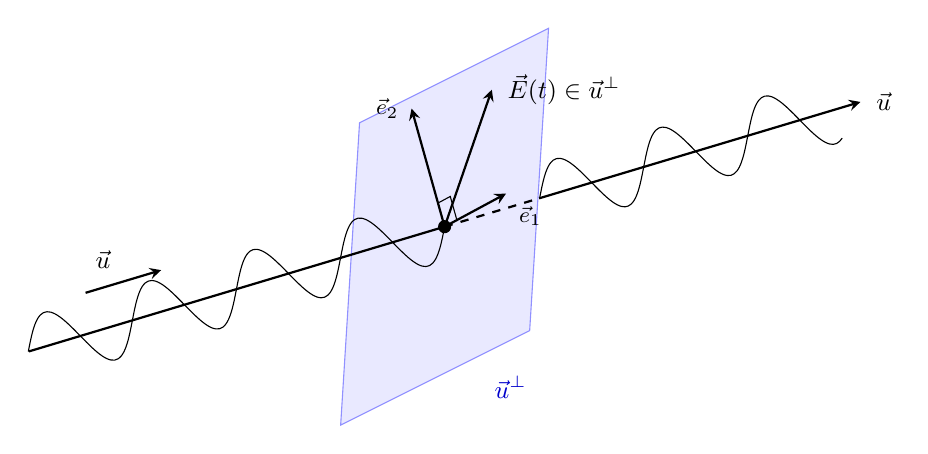
\begin{tikzpicture}[scale=1.2, >=stealth]
        % --- Points de référence de l'axe du rayon u (incliné montant) ---
        \coordinate (O)     at (0, 0);               % Centre / intersection
        \coordinate (Left)  at (-4.4, -1.32);        % Origine gauche basse
        \coordinate (Mid)   at (1.0, 0.3);           % Fin de la zone cachée
        \coordinate (Right) at (4.4, 1.32);          % Arrivée droite haute

        % ==============================================================
        % 1. PLAN ORTHOGONAL u^\bot (davantage incliné, teinté bleu)
        % ==============================================================
        % Sommets du parallélogramme basculé
        \coordinate (P1) at (-1.1, -2.1);
        \coordinate (P2) at (0.9, -1.1);
        \coordinate (P3) at (1.1, 2.1);
        \coordinate (P4) at (-0.9, 1.1);

        \filldraw[fill=blue!10, draw=blue!50, thin, opacity=0.85] 
            (P1) -- (P2) -- (P3) -- (P4) -- cycle;

        % Label du plan u^\bot
        \node[blue!80!black, font=\small] at (0.7, -1.7) {$\vec{u}^\perp$};

        % ==============================================================
        % 2. AXE DU RAYON LUMINEUX (Incliné montant vers la droite)
        % ==============================================================
        % Segment amont
        \draw[thick] (Left) -- (O);
        
        % Traversée immédiate après le centre (atténuée/pointillée)
        \draw[thick, dashed] (O) -- (Mid);
        
        % Segment aval émergeant
        \draw[thick, ->] (Mid) -- (Right) node[right=2pt, font=\small] {$\vec{u}$};

        % Flèche et label du vecteur u au départ
        \draw[thick, ->] (-3.8, -0.7) -- (-3.0, -0.46) 
            node[midway, above left=1pt, font=\small] {$\vec{u}$};

        % ==============================================================
        % 3. ONDE SINUSOÏDALE (le long de l'axe incliné)
        % ==============================================================
        % Rotation locale de l'onde pour suivre la pente (environ 16.7 degrés)
        \begin{scope}[rotate around={16.7:(O)}]
            % Onde amont (x de -4.6 à 0)
            \draw[domain=-4.6:0, samples=120, smooth, variable=\x, thin, black] 
                plot ({\x}, {0.35*sin((\x+4.6)*360/1.15)});

            % Onde aval (x de 1.05 à 4.3)
            \draw[domain=1.05:4.3, samples=90, smooth, variable=\x, thin, black] 
                plot ({\x}, {0.35*sin((\x-1.05)*360/1.15)});
        \end{scope}

        % ==============================================================
        % 4. BASE ORTHOGONALE ET VECTEUR E(t) DANS LE PLAN
        % ==============================================================
        % Vecteur e2 (direction haute du plan)
        \draw[thick, ->] (O) -- (-0.35, 1.25) node[left=1pt, font=\footnotesize] {$\vec{e}_2$};
        
        % Vecteur e1 (oblique, fuite vers la droite dans le plan)
        \draw[thick, ->] (O) -- (0.65, 0.35) node[below right=1pt, font=\footnotesize] {$\vec{e}_1$};

        % Symbole d'angle droit entre e1 et e2
        \draw[thin] (-0.07, 0.25) -- (0.06, 0.32) -- (0.13, 0.07);

        % Vecteur champ électrique E(t)
        \draw[thick, ->, black] (O) -- (0.5, 1.45) 
            node[right=2pt, font=\small] {$\vec{E}(t) \in \vec{u}^\perp$};

        % Point central d'impact O
        \filldraw[fill=black] (O) circle (1.8pt);
    \end{tikzpicture}
    \caption{Propagation libre le long de $\vec{u}$ et confinement de l'oscillation transverse $\vec{E}(t)$ dans le plan orthogonal $\vec{u}^\perp = \mathrm{Vect}(\vec{e}_1, \vec{e}_2)$.}
    \label{fig:onde_transverse_inclinee}
\end{figure}

Si l'on secoue la corde, la perturbation ondulatoire se propage vers l'avant, mais le déplacement de la corde s'effectue toujours de manière transverse (perpendiculaire à l'axe de visée). On peut secouer la corde de gauche à droite ou de bas en haut : la trajectoire du mouvement se projette alors sur le mur dans un plan orthogonal à la corde. Ce plan vectoriel de dimension 2 admet une base orthonormée $(\vec{e}_1, \vec{e}_2)$ qui permet de décomposer toute oscillation transverse arbitraire.

En transposant cette analogie à la lumière, la corde matérialise la direction de propagation $\vec{u}$. En chaque point du trajet, le champ électrique $\vec{E}(t)$ est strictement confiné dans le plan orthogonal $\vec{u}^\perp$. Les deux directions de base $(\vec{e}_1, \vec{e}_2)$ représentent les deux états de polarisation linéaire indépendants de l'onde. La fréquence temporelle d'oscillation fixe la longueur d'onde $\lambda$ (la couleur spectrale), tandis que l'amplitude du vecteur $\vec{E}(t)$ régit l'énergie transportée.

% ---------------------------------------------
\subsection{Réflexion \& Réfraction}

Les principes de réflexion et réfraction décrivent le comportement d'un faisceau traversant une discontinuité entre deux milieux aux propriétés optiques distinctes. Pour quantifier la réponse de ces milieux vis-à-vis de la lumière, on introduit la notion \emph{d'indice de réfraction}.

\begin{definition}[Indice de réfraction]
    Soit un milieu homogène et isotrope, on appelle \emph{indice de réfraction} $n$ de ce milieu le rapport adimensionnel entre la vitesse de la lumière dans le vide $c$ et la vitesse de phase $v$ de l'onde dans ce milieu :
    \begin{equation}
        n = \frac{c}{v}.
    \end{equation}
    Puisque la vitesse dans la matière vérifie $v \leqslant c$, on a généralement $n \geqslant 1$ dans le domaine optique. Plus l'indice $n$ est élevé, plus le milieu est dit \emph{réfringent} et plus la propagation de l'onde y est ralentie.
\end{definition}

Soient deux milieux d'indices respectifs $n_1$ (milieu incident) et $n_2$ (milieu de transmission). On étudie le comportement d'un rayon lumineux frappant une interface plane séparant ces deux milieux (voir Figure~\ref{fig:fresnel_polarisation_schema}).


\begin{figure}[htbp]
    \centering
    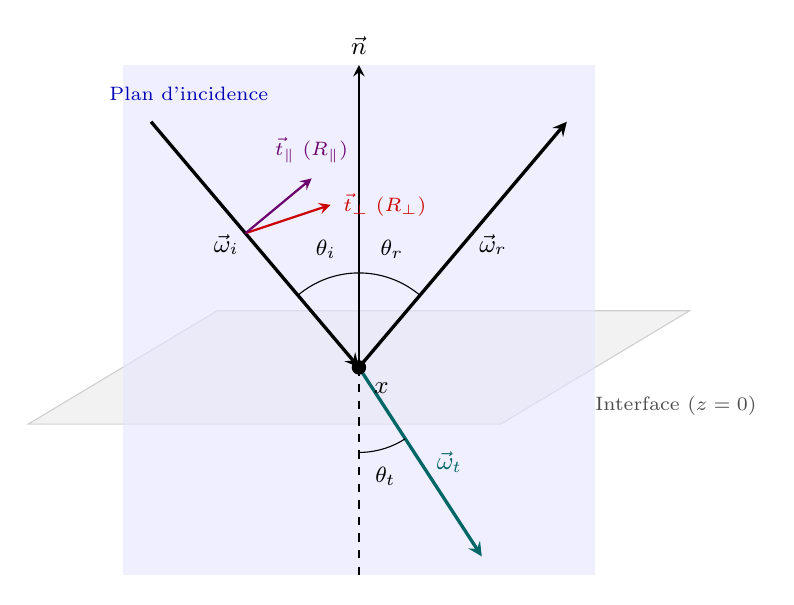
\begin{tikzpicture}[scale=1.2, >=stealth]
        % --- Interface matérielle (plan horizontal z = 0) ---
        \filldraw[fill=gray!15, draw=gray!50, opacity=0.7] 
            (-3.5, -0.6) -- (1.5, -0.6) -- (3.5, 0.6) -- (-1.5, 0.6) -- cycle;
        \node[gray!60!black, font=\scriptsize, right] at (2.4, -0.4) {Interface ($z=0$)};

        % Origine x
        \coordinate (O) at (0, 0);

        % --- Plan d'incidence (ombré en bleu translucide) ---
        \fill[blue!10, opacity=0.6] 
            (-2.5, 3.2) -- (2.5, 3.2) -- (2.5, -2.2) -- (-2.5, -2.2) -- cycle;
        \node[blue!70!black, font=\scriptsize] at (-1.8, 2.9) {Plan d'incidence};

        % --- Normale de surface ---
        \draw[thick, ->] (O) -- (0, 3.2) node[above, font=\small] {$\vec{n}$};
        \draw[thick, dashed] (0, 0) -- (0, -2.2);

        % --- Rayons lumineux ---
        % Rayon incident
        \draw[very thick, ->] (-2.2, 2.6) -- (O) node[midway, left=2pt, font=\small] {$\vec{\omega}_i$};
        % Rayon réfléchi
        \draw[very thick, ->] (O) -- (2.2, 2.6) node[midway, right=2pt, font=\small] {$\vec{\omega}_r$};
        % Rayon réfracté (transmis)
        \draw[very thick, ->, teal!80!black] (O) -- (1.3, -2.0) node[midway, right=2pt, font=\small] {$\vec{\omega}_t$};

        % --- Angles theta_i, theta_r, theta_t ---
        \draw[thin] (0, 1.0) arc (90:130:1.0);
        \node[font=\footnotesize] at (-0.35, 1.25) {$\theta_i$};

        \draw[thin] (0, 1.0) arc (90:50:1.0);
        \node[font=\footnotesize] at (0.35, 1.25) {$\theta_r$};

        \draw[thin] (0, -0.9) arc (-90:-57:0.9);
        \node[font=\footnotesize] at (0.28, -1.15) {$\theta_t$};

        % --- Décomposition de la polarisation sur le rayon incident ---
        \coordinate (P) at (-1.2, 1.42); % Point sur le rayon incident

        % Axe perpendiculaire (t_perp : hors du plan, le long de l'interface)
        \draw[thick, ->, red!80!black] (P) -- ++(0.9, 0.3) 
            node[right=1pt, font=\scriptsize] {$\vec{t}_\perp$ ($R_\perp$)};

        % Axe parallèle (t_parallel : dans le plan d'incidence, orthogonal au rayon)
        \draw[thick, ->, violet!85!black] (P) -- ++(0.7, 0.58) 
            node[above=2pt, font=\scriptsize] {$\vec{t}_\parallel$ ($R_\parallel$)};

        % Point de contact
        \filldraw[fill=black] (O) circle (2pt) node[below right=2pt, font=\small] {$x$};
    \end{tikzpicture}
    \caption{Décomposition des composantes de polarisation orthogonale ($R_\perp$) et parallèle ($R_\parallel$) par rapport au plan d'incidence.}
    \label{fig:fresnel_polarisation_schema}
\end{figure}



Le rayon incident est modélisé par sa direction unitaire $\vec{\omega}_i$, faisant un angle $\theta_i \in [0, \frac{\pi}{2}]$ avec la normale sortante $\vec{n}$ à l'interface. L'interaction génère deux composantes :
\begin{itemize}
    \item un rayon réfléchi $\vec{\omega}_r$, dont l'angle vérifie la loi de réflexion spéculaire $\theta_r = \theta_i$ ;
    \item un rayon réfracté (ou transmis) $\vec{\omega}_t$, dont l'angle $\theta_t$ dans le second milieu est dicté par la loi de Snell-Descartes :
    \begin{equation}
        n_1 \sin\theta_i = n_2 \sin\theta_t.
    \end{equation}
\end{itemize}

\begin{remark}[Réflexion totale interne]
    Lorsque le faisceau se propage d'un milieu plus réfringent vers un milieu moins réfringent ($n_1 > n_2$), la quantité $\frac{n_1}{n_2}\sin\theta_i$ peut excéder $1$. Il existe alors un angle critique $\theta_c = \arcsin\left(\frac{n_2}{n_1}\right)$ au-delà duquel aucun rayon ne peut être transmis dans le second milieu : toute l'énergie est réfléchie dans le premier milieu (\emph{réflexion totale interne}).
\end{remark}

\begin{proposition}[Décomposition géométrique de la polarisation]
    Pour analyser l'oscillation du champ électrique transverse $\vec{E} \in \vec{\omega}_i^\perp$, la présence de la surface brise l'isotropie spatiale et impose un plan de référence. Deux vecteurs non colinéaires $\vec{\omega}_i$ et $\vec{n}$ définissent le \emph{plan d'incidence} $\mathcal{P} = \operatorname{Vect}(\vec{\omega}_i, \vec{n})$.

    Le plan des oscillations permises $\vec{\omega}_i^\perp$ admet alors une décomposition canonique en deux directions orthogonales :
    \begin{enumerate}
        \item \textbf{Direction orthogonale $\vec{t}_\perp$ (polarisation $s$)} : perpendiculaire au plan d'incidence $\mathcal{P}$, obtenue par produit vectoriel :
        \begin{equation}
            \vec{t}_\perp = \frac{\vec{\omega}_i \times \vec{n}}{\|\vec{\omega}_i \times \vec{n}\|}.
        \end{equation}
        Ce vecteur est par construction orthogonal à $\vec{n}$ : il oscille parallèlement à l'interface matérielle.
        \item \textbf{Direction parallèle $\vec{t}_\parallel$ (polarisation $p$)} : contenue dans le plan d'incidence $\mathcal{P}$ et orthogonale à la direction de propagation $\vec{\omega}_i$ :
        \begin{equation}
            \vec{t}_\parallel = \vec{\omega}_i \times \vec{t}_\perp.
        \end{equation}
    \end{enumerate}
    Toute onde incidente se projette de façon unique sur cette base : $\vec{E}_i = E_\perp \vec{t}_\perp + E_\parallel \vec{t}_\parallel$.
\end{proposition}

\begin{proposition}[Équations de Fresnel et bilan énergétique]
    La conservation de l'énergie impose que la somme de la réflectance $R$ et de la transmittance $T$ vaille $1$. Les équations de Fresnel fournissent les coefficients de réflexion énergétique exacts pour chacune des deux polarisations :
    \begin{align}
        R_\perp(\theta_i) &= \left( \frac{n_1 \cos\theta_i - n_2 \cos\theta_t}{n_1 \cos\theta_i + n_2 \cos\theta_t} \right)^2 = \left( \frac{\sin(\theta_i - \theta_t)}{\sin(\theta_i + \theta_t)} \right)^2, \label{eq:fresnel_perp} \\
        R_\parallel(\theta_i) &= \left( \frac{n_2 \cos\theta_i - n_1 \cos\theta_t}{n_2 \cos\theta_i + n_1 \cos\theta_t} \right)^2 = \left( \frac{\tan(\theta_i - \theta_t)}{\tan(\theta_i + \theta_t)} \right)^2. \label{eq:fresnel_para}
    \end{align}
\end{proposition}

En synthèse d'images, la lumière naturelle et les sources d'éclairage sont modélisées comme non polarisées : les directions d'oscillation dans $\vec{\omega}_i^\perp$ sont réparties de manière isotrope. Le coefficient de Fresnel effectif $F(\theta_i)$ est la moyenne équipondérée des deux modes ($s = p = 0{,}5$) :
\begin{equation}
    F(\theta_i) = \frac{R_\perp(\theta_i) + R_\parallel(\theta_i)}{2}.
\end{equation}

\begin{proposition}[Approximation de Schlick]
    Pour éviter l'évaluation trigonométrique coûteuse des équations~(\ref{eq:fresnel_perp}) et~(\ref{eq:fresnel_para}) lors du tracé de rayons, on utilise l'approximation polynomiale de Schlick :
    \begin{equation}
        F(\theta_i) \approx R_0 + (1 - R_0)(1 - \cos\theta_i)^5
    \end{equation}
    où $R_0$ représente la réflectance mesurée à incidence normale ($\theta_i = 0$, soit $\cos\theta_i = 1$) :
    \begin{equation}
        R_0 = \left( \frac{n_1 - n_2}{n_1 + n_2} \right)^2.
    \end{equation}
\end{proposition}

Cette approximation reproduit fidèlement deux propriétés physiques majeures :
\begin{itemize}
    \item À incidence normale ($\theta_i \approx 0$), la réflectance vaut $R_0$ (typiquement de l'ordre de $0{,}04$ pour des matériaux tels que verre et l'eau);
    \item À incidence rasante ($\theta_i \to \frac{\pi}{2}$, $\cos\theta_i \to 0$), le terme $(1 - \cos\theta_i)^5 \to 1$, d'où $F(\theta_i) \to 1$ : toute surface devient un réflecteur parfait aux angles rasants.
\end{itemize}

% ---------------------------------------------
\subsection{Fonction de distribution de la réflectance bidirectionnelle - BRDF}

Les modèles vus précédement caractérisent la réponse locale d'une interface plane et optiquement lisse, où la réflexion est exclusivement spéculaire. Pour modéliser des matériaux macroscopiques réels présentant de la rugosité ou des phénomènes de diffusion interne, il est nécessaire d'introduire un formalisme reliant l'irradiance incidente à la radiance réémise dans chaque direction de l'espace.
Ici, nous commençons par présenter le modèle général puis proposons une simplification utilisant des lois de probabilités. 

Dans le cas le plus général, le transport de lumière à une frontière matérielle est un phénomène continu à 12 dimensions :
\begin{equation}
    S(x_i, \vec{\omega}_i, t_i, \lambda_i \;\to\; x_r, \vec{\omega}_r, t_r, \lambda_r)
\end{equation}
où $x_i, x_r$ sont les positions spatiales d'entrée et de sortie, $\vec{\omega}_i, \vec{\omega}_r$ les directions sphériques correspondantes, $t_i, t_r$ les instants d'interaction, et $\lambda_i, \lambda_r$ les longueurs d'onde associées.

\begin{proposition}[Simplification]
    En synthèse d'images usuelle, trois hypothèses simplificatrices sont admises :
    \begin{itemize}
        \item \textbf{Indépendance temporelle} ($t_i = t_r$) : la vitesse de propagation est considérée infinie à l'échelle de la scène, excluant les effets de phosphorescence.
        \item \textbf{Cohérence spectrale} ($\lambda_i = \lambda_r$) : la lumière réfléchie conserve sa longueur d'onde incidente, excluant la fluorescence.
        \item \textbf{Hypothèse de localité spatiale} ($x_i \approx x_r = x$) : pour les matériaux opaques, la distance de diffusion interne sous la surface est négligeable devant les échelles macroscopiques. La fonction de diffusion sous-surfacique (BSSRDF, en dimension 8) se réduit alors à une fonction locale définie en un unique point matériel $x$.
    \end{itemize}    
\end{proposition}

Cette réduction dimensionnelle aboutit à la \emph{Bidirectional Reflectance Distribution Function} (BRDF), fonction à quatre paramètres angulaires $(\theta_i, \phi_i, \theta_r, \phi_r)$ paramétrée par la longueur d'onde $\lambda$.

\begin{definition}[BRDF]
    Soit un point $x$ sur une surface, la BRDF, notée $f_r$, est le rapport différentiel entre la radiance réfléchie $\dd L_r$ dans la direction $\vec{\omega}_r$ et l'irradiance incidente différentielle $\dd E_i$ arrivant depuis le secteur solide élémentaire $\dd\omega_i$ autour de $\vec{\omega}_i$ :
    \begin{equation}
        f_r(x, \vec{\omega}_i, \vec{\omega}_r, \lambda) = \frac{\dd L_r(x \to \vec{\omega}_r, \lambda)}{\dd E_i(x \leftarrow \vec{\omega}_i, \lambda)} = \frac{\dd L_r(x \to \vec{\omega}_r, \lambda)}{L_i(x \leftarrow \vec{\omega}_i, \lambda) \cos\theta_i \, \dd\omega_i}.
    \end{equation}
    Elle s'exprime en stéradians inverses ($\mathrm{sr}^{-1}$).
\end{definition}

\begin{prop}[Fondamentales]
    Pour être physiquement admissible, tout modèle mathématique de BRDF doit impérativement respecter deux contraintes thermodynamiques :
    \begin{enumerate}
        \item \textbf{Réciprocité d'Helmholtz} : la fonction de transfert optique est invariante par inversion du sens de parcours de la lumière :
        \begin{equation}
            f_r(x, \vec{\omega}_i, \vec{\omega}_r, \lambda) = f_r(x, \vec{\omega}_r, \vec{\omega}_i, \lambda).
        \end{equation}
        Cette propriété garantit l'équivalence entre les algorithmes traçant les rayons depuis l'observateur (\emph{path tracing}) et ceux partant des sources de lumière (\emph{ligh-tracing}).
        \item \textbf{Conservation de l'énergie} : une surface passive ne pouvant amplifier l'énergie incidente, la puissance totale réémise sur l'hémisphère supérieur $\Omega^+$ ne peut excéder la puissance reçue. Pour toute direction incidente $\vec{\omega}_i$ :
        \begin{equation}
            \int_{\Omega^+} f_r(x, \vec{\omega}_i, \vec{\omega}_r, \lambda) \cos\theta_r \, \dd\omega_r \leqslant 1.
        \end{equation}
    \end{enumerate}
\end{prop}

% Les modèles de réflectance se divisent canoniquement en deux approches :
% \begin{itemize}
%     \item \textbf{Modèles implicites (phénoménologiques ou projectifs)} : ils font abstraction de la géométrie locale et approximent le comportement lumineux via des formulations empiriques ou analytiques simples (modèles de Lambert, Phong, Blinn-Phong).
%     \item \textbf{Modèles explicites (microfacettes)} : ils modélisent explicitement la rugosité de la surface sous la forme d'une distribution statistique de facettes microscopiques lisses orientées selon une densité de normales. La réponse globale intègre alors les fonctions de masquage/ombrage géométrique $G$, la distribution des normales $D$ et le terme de Fresnel spéculaire $F$ (modèles de Cook-Torrance, Beckmann, GGX).
% \end{itemize}